%%This is a very basic article template.
%%There is just one section and two subsections.
\RequirePackage[ngerman=ngerman-x-latest]{hyphsubst}
%\documentclass[11pt,a4paper]{scrbook}
\documentclass[11pt,a4paper]{scrartcl}
%\documentclass[11pt,a4paper]{article}
\usepackage[utf8]{inputenc}
\usepackage[T1]{fontenc}
%\renewcommand{\familydefault}{\sfdefault}
\usepackage[a4paper]{geometry}
%\geometry{verbose,tmargin=2.5cm,lmargin=2.5cm,rmargin=1.5cm,bmargin=3cm}
\usepackage[ngerman,english]{babel}
%\usepackage{ngerman}
\usepackage{amsmath}
\usepackage{mhchem}
\usepackage{textcomp}
\usepackage{amsfonts}
\usepackage{amssymb}
\usepackage{setspace}
\usepackage[pdftex]{graphicx}
\usepackage{epstopdf}
\usepackage[final]{pdfpages}
\usepackage{booktabs}
\usepackage{multirow}
%\usepackage{chngcntr}
%\usepackage{hyperref}0
\usepackage{placeins}

\setlength{\parindent}{0pt}
\setlength{\headheight}{14pt}
\usepackage{fancyhdr}
\pagestyle{fancy}
\begin{document}

\begin{titlepage}
\begin{center}

\includegraphics[scale=0.8]{images/HSR.pdf}
\linebreak 
\includegraphics[scale=0.3]{images/IET.pdf}
\end{center}

\vspace{2.5cm}
%\vspace{0.5cm}
\begin{center}
\textbf{Latentwärmespeicher und chemische Speicher
in Gebäudeenergieversorgungssystemen}
\linebreak
%\textbf{evtl. Vertraulich}
\end{center}
\vspace{1.8cm}
%\vspace{0.5cm}
\begin{center}
Seminararbeit
\end{center}
\vspace{1cm}
\begin{center}
\textbf{von \linebreak Dominik Strebel \linebreak Simon Boller \linebreak
Leandro Nikolic} \linebreak
\linebreak 
Abgabedatum: 23.05.2014
\linebreak
\end{center}
\vspace{3cm}
\noindent Betreuung:

\noindent Prof. Carsten Wemhöner

\noindent HSR Rapperswil

\noindent Institut für Energietechnik

\end{titlepage}
%\thispagestyle{empty}
%\cleardoublepage
\renewcommand{\footrulewidth}{0pt}
\renewcommand{\headrulewidth}{0pt}
\lhead{}
\chead{}
\rhead{}
\cfoot{} 
\selectlanguage{ngerman}


 \vspace*{12.5cm}
\begin{minipage}{80mm}
	Keywords: Wärmespeicher, Latentwärmespeicher, chemische Speicher
 \\
	\\
	Zitiervorschlag: 
	Ich beschäftige mich nicht mit dem, was getan worden ist. Mich interessiert, was getan werden muss. Marie Curie
	\vspace{1cm}


  \rule{80mm}{2pt}
  Impressum: \\
  Hochschule für Technik Rapperswil \\
  IET, Institut für Energietechnik \\ 
  Oberseestrasse 10 \\
  8640 Rapperswil\\
  \rule{80mm}{2pt}
\end{minipage}
\newpage


\tableofcontents
\newpage
\renewcommand{\headrulewidth}{0.4pt}
\renewcommand{\footrulewidth}{0.4pt}
\lhead{}
\chead{Seminararbeit}
\rhead{}
\cfoot{}
\setcounter{page}{1}
\cfoot{\thepage}
\section{Einleitung}
\newpage
\section{Allgemeiner Vergleich von chemischen, latenten und sensiblen
Wärmespeichern}
Wärmespeicher lassen sich generell in zwei verschiedene Hauptgruppen einteilen.
Einerseites existieren chemische Energiespeicher, andererseits
direkt-thermische, in denen die Energie ohne Umwandlung als thermische Energie
verfügbar ist. Eine Gliederung der verschiedenen Technologien befindet sich in
der Abbildung
\ref{fig:Wärmespeicher}

\begin{figure}[h]
\begin{center}
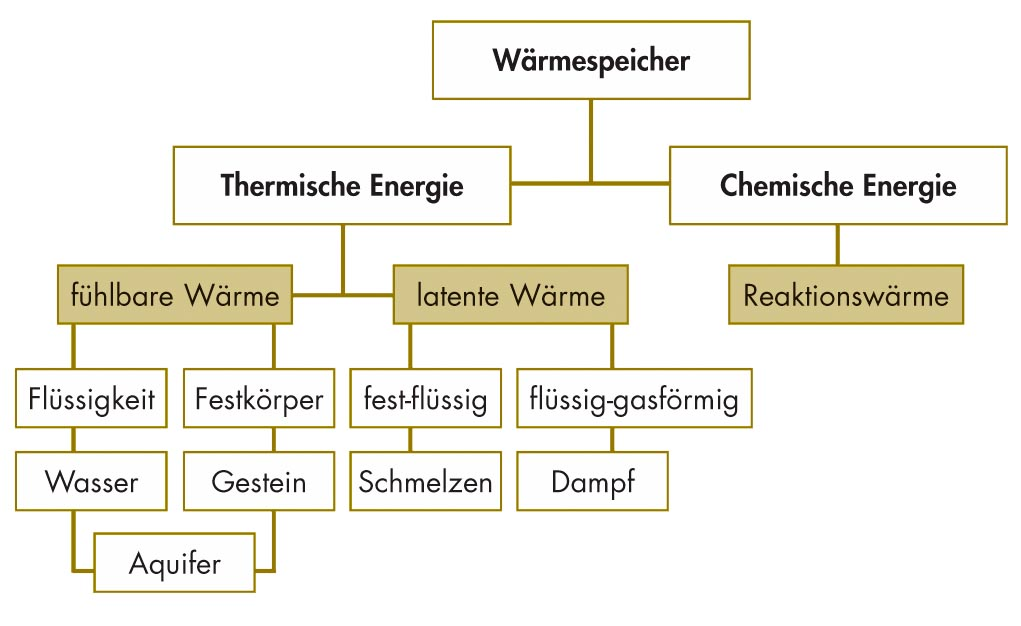
\includegraphics[scale=0.3]{images/speicher.jpg}
\caption{Übersicht über die verschiedenen Wärmespeichertechnolgien \cite{BINE1}}
\label{fig:Wärmespeicher}
\end{center}
\end{figure}

\subsection{Chemische Speicher}
Chemische Speicher werden über eine chemsiche Reaktion be- und entladen. Per
Definition eines Speichers sind diese Reaktionen reversibel. Die nutzbare
Wärmeenergie entspricht der freigesetzten Reaktionsenthalpie $\Delta
H_{\mathrm{R}}$. Die Nutztemperatur des Speichers bestimmt die in Frage
kommenden chemischen Reaktionen und schränkt die zu verwenden Stoffe erheblich
ein.

Chemische Speicher werden heute im allgemeinen mit sorptiven Prozessen gebaut.
Dies ist einerseits die Adsorption, eine Anlagerung eines Gases oder einer
Flüssigkeit an einen Feststoff und andererseits die Absorption, das Lösen von
Gasen in einer Flüssigkeit. In untenstehender Gleichung ist das Grundlegende
Prinzip der Adsorption erklärt.
\begin{align}
\text{Sorbens}+nH_2O\leftrightharpoons \text{Sorbens}+nH_2O+\Delta H_{ads}
\end{align}
Nutzbar ist die freiwerdende Reaktionsenthalpie $\Delta H_{ads}$ wenn die
Reaktion nach links erfolgt. Die Beladung erfolgt nach umgekehrten Prinzip.  
\cite{Wesselak}

\subsection{Latente Speicher}
Latentwärmespeicher nutzen den Phasenübergang eines Stoffs zur Speicherung von
Wärme. Wie bei den chemischen Speichern beschränken sich die Einsatzgebiete auf
die Phasenübergangseigenschaften des Mediums. Beispielsweise erfolgt der
Phasenübergang von Wasser bei 273.15K. Die freiwerdende bzw. benötigte Energie
für einen fest-flüssig Phasenübergang bei Wasser beträgt 333.5 kJ/kg.
Aufgrund der grossen Dichteänderund der meisten flüssig-gasförmig
Phasenübergänge werden diese selten zu Speicherzwecken genutzt, obwohl die
Kondensations/Verdampfungswärme der Stoffe meistens grösser ist. Die Materialien
werden mit PCM für \flqq Phase Changing Materials\frqq{} abgekürzt.

Die speicherbare Energie ergibt sich nach

\begin{align}
\Delta E = mh_{pc}
\end{align}
Produkt von Masse und Schmelz/Kristallisationsenthalpie. Die verwendeten
Materialien lassen sich zweidimensional anhand der
Schmelz/Kristallationsenthalpie und der Schmelztemperatur kategorisieren. 

Nachteilig bei Latentwärmespeichern ist besonders, dass bei reinen Feststoffen
naturgemäss kein konvektiver Wärmetransport stattfinden kann. Dem versucht man
im heutigen Forschungskontext mit sogennaten Slurries zu begegnen. Im weiteren
Verlauf dieser Arbeit werden wir darauf noch eingehen. \cite{Wesselak}

\subsection{Sensible Wärmespeicher}

Sensible Wärmespeicher funtkionieren klassisch über eine Temperaturdifferenz
$\Delta T$. Sensibel bedeutet in diesem Kontext \flqq fühlbar\frqq{}. Die
Be- und Entladung funktioniert also über einen \flqq fühlbare\frqq{}
Temperaturdifferenz die über konvektive und konduktive Prozesse zum Austausch
führt. Als Speichermedium eignen sich aufgrund von Dichteeigenschaft und
gewünschter Konvektion verschiedene Flüssigkeiten. Die spezifische
Wärmekapazität $c$ und die Speichermasse $m$ bestimmen die Kapazität des
Speichers, der Massenstrom $\dot{m}$ und Temperaturdifferenz $\Delta T$ die
Leistung des Speichers. Aufgrund der auch an den Speicherwänden anliegenden
Temperaturdifferenz $\Delta T$ ist eine Dämmung zwingend notwendig. 

Technisch gesehen unterscheidet man zwischen Kurz- und Langzeitspeichern.
Typischer Kurzzeitspeicheranwendungen im Gebäudetechnikbereich sind
Warmwasserboiler. Die Verweildauer des Wassers beträgt hier Stunden bis maximal
Tasge. Langzeitspeicher werden zur saisonalen Wärmespeicherung genutzt. Dies
findet beim System Jenni Einsatz. Die Speicher sind so dimensioniert, dass die
SPeicherkapazität nur ein- bis wenige Male im Jahr genutzt wird. Dafür sind aber
grosse Speichermassen, bis zu 100'000l Wasser nötig.

Die gespeicherte Energiemenge lässt sich nach
\begin{align}
\Delta E = mc\Delta T = \rho Vc \Delta T
\end{align}
definieren. Wasser besitzt mit 4.19 kJ/kg/K eine hohe spezifische
Wärmekapazität und wird deshalb als kostengünstiges, effizientes und
umweltfreundliches Medium omnipräsent eingesetzt.
In Abbildung \ref{fig:Langzeitspeicher} sind die verfügbaren
Langzeitsenisbelwärmespicher abgebildet. D

\begin{figure}[h]
\begin{center}
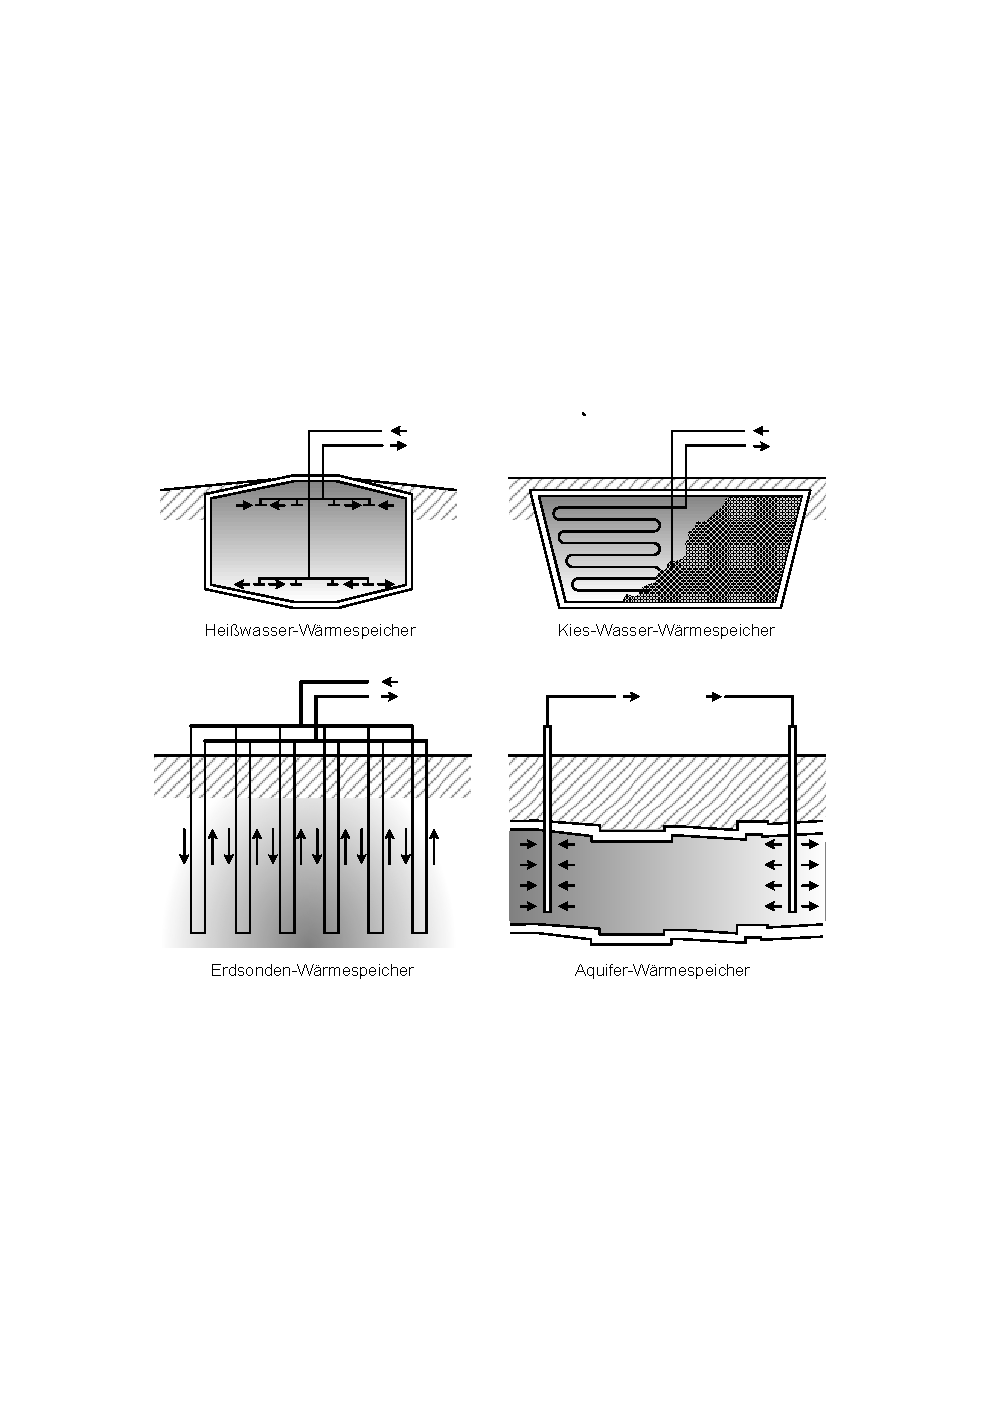
\includegraphics[scale=1]{images/langzeitspeicher.pdf}
\caption{Langzeitsensibelwärmespeicher \cite{Wesselak}}
\label{fig:Langzeitspeicher}
\end{center}
\end{figure}

\section{Technologischer Überblick}
In diesem Kapitel werden der Stand der Technik, die Entwicklung, Perspektiven
und Herausforderungen der zwei zu behandelnden Speichertechnologien erläutert.
\subsection{Latentspeicher}
In den folgenden Unterkapiteln wird ein allgemeiner Überblick über
Latentwärmespeicher gegeben und danach spezifisch auf den Stand der Technik und
die zukünftige Entwicklung eingegangen.
\subsubsection{Allgemein}
Latentspeicher nützen den Phasenwechsel aus. Jedes Material besitzt einen
sogenannten Schmelz- bzw. Erstarrungspunkt und einen Siede- bzw.
Kondensationspunkt. An diesem Temperaturpunkt wechselt das Medium sine Phase von
fest zu flüssig bzw. von flüssig zu gasförmig. Um diese Phasenänderung
vorzunehmen benötigt das Medium viel Wärmeenergie bzw. gibt viel Wärmeenergie an
die Umgebung ab. Das Beispiel in Abbildung \ref{fig:H2O} zeigt die Benötigte
Wärmeenergie für die Temperaturerhöhung und den Phasenübergang von Wasser bei
Normdruck auf.

\begin{figure}[h!]
\begin{center}
\includegraphics[scale=0.6]{images/Phasendiagramm.pdf}
\caption{Phasenübergänge von \ce{H_2O} und die dafür benötigten Energiemengen}
\label{fig:H2O}
\end{center}
\end{figure}
Deutlich zu erkennen ist einerseits die enorm grosse Schmelz- und
Verdampfungswärme im Vergleich zu der temperaturerhöhenden Wärme. Zu
berücksichtigen ist dabei, dass die X-Achse nicht linear verläuft. Andererseits
ist ersichtlich, dass die zum Phasenwechsel benötigte Wärme auf demselben
Temperaturniveau stattfindet. Die Schmelz- und Verdampfungswärme wird auch als
latente Wärme bezeichnet. Die restliche Wärme, welche eine Temperaturdifferenz
hervorruft wird sensible Wärme genannt.
Der Temperaturpunkt, an welchem der Phasenübergang stattfindet ist vom Medium
und vom herrschenden Druck abhängig. Abbildung \ref{fig:H2O2} zeigt das
Phasendiagramm von Wasser. Erkennbar ist, dass der Schmelz- und Siedepunkt sich
mit Veränderung des Druckes ebenfalls ändern
\begin{figure}[h!]
\begin{center}
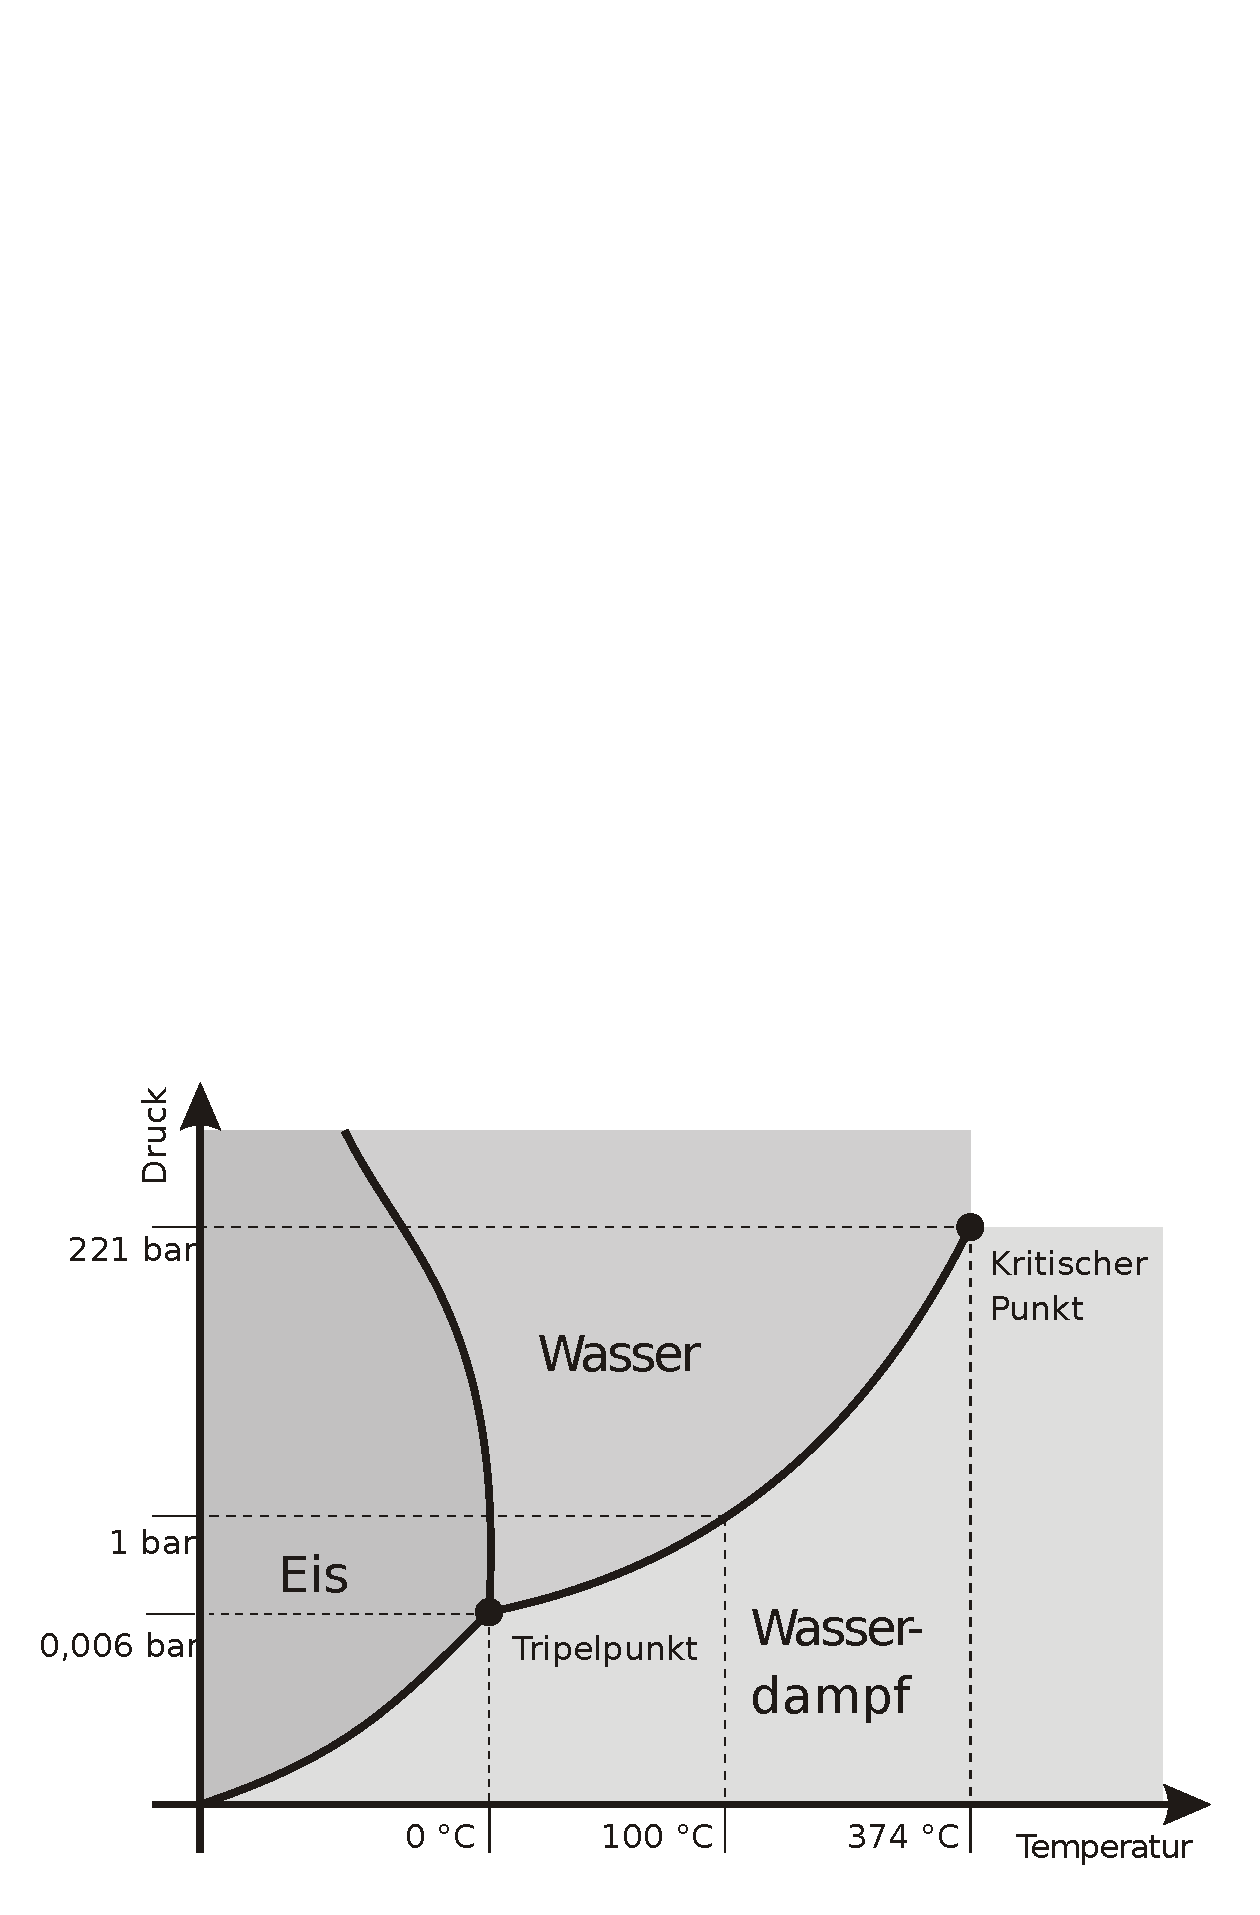
\includegraphics[scale=0.6]{images/Phasendiagramm2d.pdf}
\caption{Phasendiagramm von \ce{H_2O} \cite{Phasendiagramm}}
\label{fig:H2O2}
\end{center}
\end{figure}
Bei einem Latentwärmespeicher versucht man somit ein Medium unter einem gewissen
Druck zu halten, damit dieses einen Phasenwechsel vornimmt bei einer gewünschten
Temperatur. Dadurch kann viel Energie bei keinem Temperaturhub gespeichert
werden. Mit der untenstehenden Formel lässt sich die speicherbare Energie
einfach berechnen:

\begin{align}
\Delta Qv = m \cdot (\Delta U + p \cdot \Delta V) = m \cdot \Delta Hv
\label{eq:latent}
\end{align}

\begin{table}[h!]
\begin{center}
\begin{tabular}{|l|p{5cm}|l|}
\hline $\Delta Qv$ & Schmelz- bzw. Verdampfungswärme & [J] \\
\hline $m$ & Masse & [kg] bzw [mol] \\
\hline $\Delta Hv$ & Spezifische Schmelz- bzw. Verdampfungsentalphie & [J/kg]
bzw. [J/mol] \\
\hline
\end{tabular}
\caption{Variablen der Gleichung \ref{eq:latent}}
\end{center}
\end{table}

Dabei hängt die Masse von der Grösse des Speichers ab und die spezifische
Enthalpie ist Mediumsabhängig.


\subsubsection{Stand der Technik}
Im Gegensatz zu sensiblen Wärmespeicher, werden Latentwärmespeicher weniger
häufig eingesetzt. Wie Tabelle \ref{tab:Wesselak1} zeigt sind verschiedene
Latentspeicher entwickelt aber noch nicht ausgereift.

\begin{table}[h]
\begin{center}
\caption{Speicherkapazität und Entwicklungsstand thermischer Speicher
\cite{Wesselak} S.682}
\label{tab:Wesselak1}
\begin{tabular}{@{}lp{2cm}p{3cm}p{2.7cm}l@{}}
\toprule
                  Speicherart & Stoff & Arbeitstemperatur \newline[$^{\circ}
                  C$]& Speicherkapazität \newline [kWh/m$^3$] &
                  Entwicklung
                  \\
                  \toprule \multirow{2}{*}{Sensibel} & Wasser  & 0-100 & 60 &
                  ausgereift
                  \\
                  & Beton & 0-500 & 30 & ausgereift  \\ \hline
\multirow{3}{*}{Latent} &Paraffine  & 0-70 & 60  & entwickelt  \\
                  & Salzhydrate & 30-100 & 150 & entwickelt \\
                  & Salze  & 100-400 & 100 & entwickelt \\ \hline
\multirow{3}{*}{Thermochemisch} & Silikagele & 40-100 & 200 & in Entwicklung  \\
                  & Zeolithe & 100-300  & 200 & in Entwicklung \\
                  & Metallhydride & 300-900 & 500 & in Entwicklung  \\ \toprule
\end{tabular}
\end{center}
\end{table}
Bei der Entwicklung von Latentwärmespeicher geht es vorwiegend um die
Herstellung eines optimalen Speichermediums. Dieses muss neben der möglichst
hohen spezifischen Phasenumwandlungsenthalpie noch viele weitere Kriterien
einhalten. Einige Anforderungen sind gemäss \cite{Wesselak} die folgenden:
\begin{itemize}
  \item Die Phasenwechseltemperatur muss im geforderten Arbeitsbereich liegen.
 \item Der Stoff sollte eine möglichst hohe spezifische
  Phasenumwandlungsenthalpie haben, damit je Masseeinheit des Speicherstoffes eine möglichst grosse
Wärmemenge gespeichert wird.
\item Der Stoff sollte eine möglichst hohe Dichte haben, um ein hohes
volumenbezogenes Speichervermögen aufzuweisen.
\item Der Stoff sollte eine hohe spezifische Wärmekapazität haben, da in der Regel
Energie auch als sensible Wärme gespeichert wird.
\item Der Stoff sollte eine möglichst hohe Wärmeleitfähigkeit besitzen, damit eine
Wärmeübertragung schon bei kleinen Temperaturdifferenzen mit relevanten
Leistungen möglich ist.
\item Der Stoff sollte ein kongruentes Schmelzverhalten haben und ohne feste
Zwischenphasen direkt aus dem festen Zustand in die homogene Schmelze übergehen
und umgekehrt. Andernfalls könnte es im Verlauf eines oder mehrerer Zyklen zu
Entmischungen und einer Abnahme der Wärmespeicherkapazität kommen.
\item Der Stoff sollte eine möglichst kleine Volumenänderung beim Phasenwechsel
aufweisen, um die mechanischen Belastungen für Speicherraum und Peripherie
möglichst gering zu halten.
\item Der Stoff sollte nicht zu Unterkühlungen neigen.
\item Der Stoff sollte chemisch und physikalisch in dem geforderten
Temperaturbereich langzeitstabil sein.
\item Der Stoff sollte keinen eng zusammen liegenden Schmelz- und Siedepunkt haben,
damit es nicht zur Verdampfung bei einer möglichen Überhitzung über den
Schmelzpunkt hinaus kommen kann.
\item Der Stoff sollte nicht korrosiv auf die verwendeten Konstruktionsmaterialien
wirken.
\item  Der Stoff darf weder toxisch, noch entflammbar oder explosiv sein. Hinzu
kommen ökonomische und ökologische Anforderungen wie die Verfügbarkeit in
grossen Mengen, ein möglichst niedrigerer Preis, Umweltverträglichkeit,
Recyclingfähigkeit und Wiederverwendbarkeit nach Erreichen der Nutzungsdauer des
Wärmespeichers.
\end{itemize}
Viele Medien befinden sich heutzutage noch in der Entwicklung. Für den
Gebäudebereich, wo häufig eine Speichertemperatur von ca. 65°C erwünscht ist,
ist das Speichermedium Natriumhydroxid-Monohydrat (\ce{NaOH - H_2O}) das
beliebteste Medium. Es weist für diesen Temperaturbereich die günstigsten
Gesamteigenschaften auf und ist bereits gut erforscht. Auch andere
Speichermedien sind bereits erforscht, haben jedoch teilweise andere
Eigenschaften und Schmelzpunkte beim selben Druck. Einige davon sind in Tabelle
\ref{tab:salz} aufgelistet.

\begin{table}[h!]
\begin{center}
\caption{Vergleich von Speichersalzsystemen für den Temperaturbereich von 0-100
$^\circ$C \cite{Wesselak}}
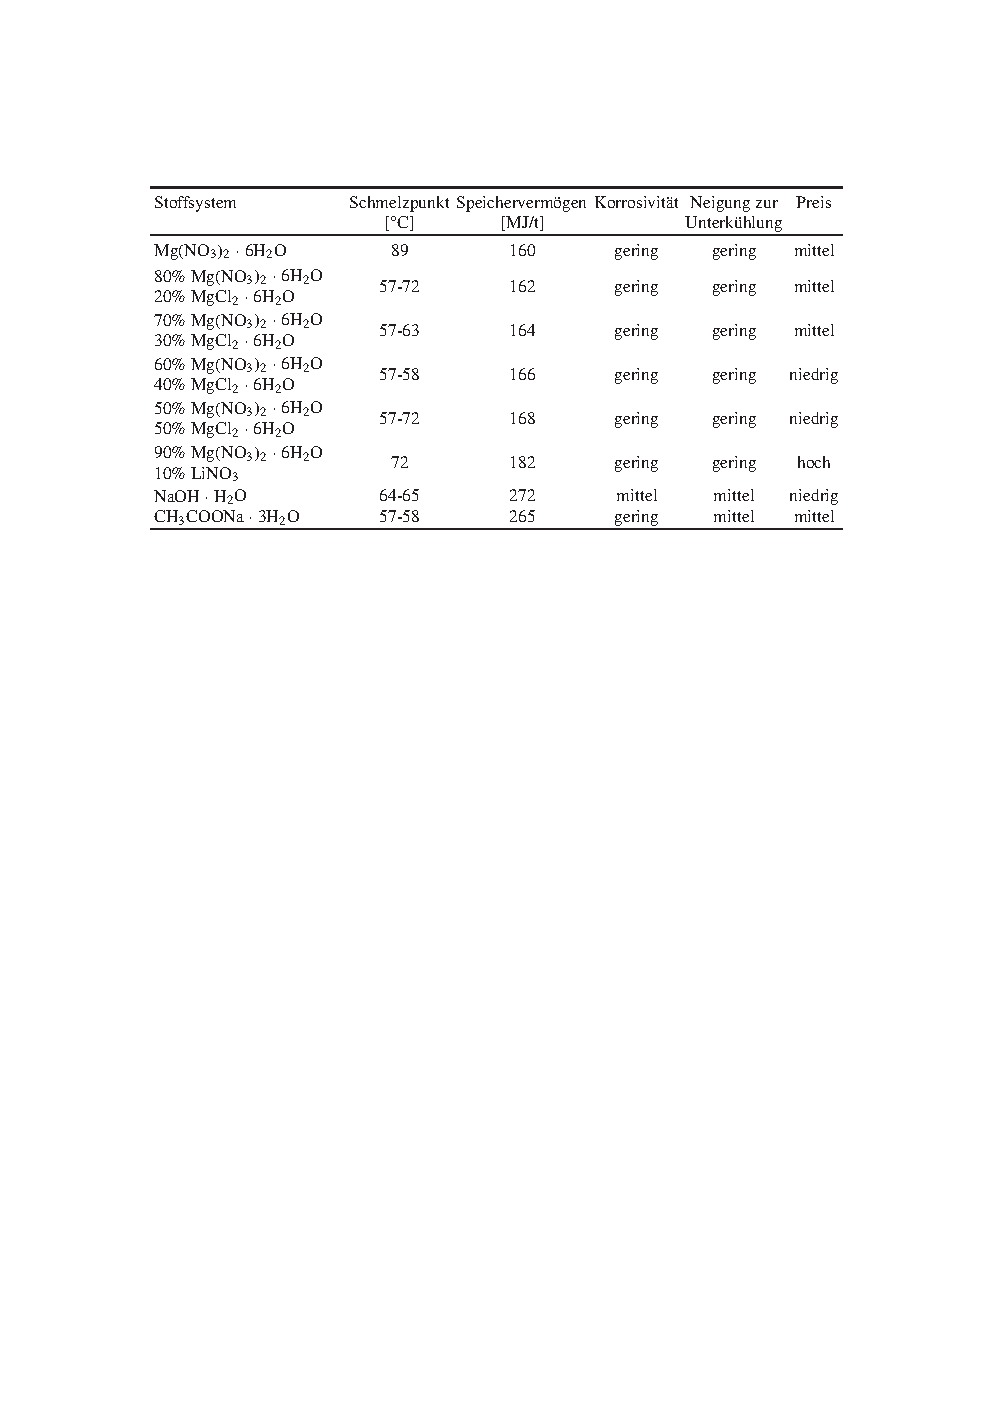
\includegraphics[scale=1]{images/speichersalze.pdf}
\label{tab:salz}
\end{center}
\end{table}
Die Hauptprobleme, welche man mit Forschungs- und Entwicklungsprojekte beheben
möchte, sind einerseits die schlechte Leitfähigkeit von Phase Change Material
(PCM). Andererseits ist es die Unterkühlung der Salzhydrate. Unterkühlung
bedeutet, dass der Phasenwechsel von Flüssig zu Fest erst bei einer zu tiefen
Temperatur stattfindet und somit eine thermodynamische Entwertung der
gespeicherten Energie vorliegt. Das erstgenannte Problem versucht man durch eine
Verkapselung und somit Vergrösserung der Oberfläche zu lösen. Den erwähnten
Unterkühlungseffekt versucht man durch das Zusetzen von Keimbildnern zu
verhindern.

Forschung wird ebenfalls betrieben um die Speicherkapazität von Gebäuden zu
erhöhen. Dies ist derzeit das grösste Einsatzfeld von PCM. Dafür wird  PCM in
die Baustoffe integriert. Solche Materialien sind heutzutage bereits kommerziell
erhältlich und werden eingesetzt.


\subsubsection{Entwicklung und Perspektiven}
Bis heute ist es noch nicht gelungen, Salzhydrate in Mikrokapseln einzubinden.
Dies versucht man jedoch in Zukunft zu ändern, um die Vorteile von Salzhydraten
gegenüber Paraffinen auszunutzen. Diese sind höhere Schmelzenthalpie und
Unentflammbarkeit. Weiter sollen durch Forschungsprojekte die Materialkosten
gesenkt und die Energiedichten erhöht werden. Die heutzutage noch fehlende
Langzeiterfahrung und die erhöhten Kosten zur Effizienzsteigerung im Gegensatz
zu sensiblen Wärmespeicher im Gebäudeeinsatz lässt die Wirtschaftlichkeit von
latenten Wärmespeichern in Frage stellen. Verschiedene Forschungsprojekte
möchten jedoch einen wirtschaftlichen Vorteil gegenüber sensiblen Speichern
erreichen.

\subsection{PCM Slurries}
In diesem Kapitel werden thermodynamische Eigenschaften von PCM-Slurries
aufgezeigt und mit denen von Wasser verglichen.
\subsubsection{Thermodynamischer Sachverhalt}
Heutzutage werden die meisten Gebäude mit einem Wassersystem geheizt und
gekühlt. Wasser wird aus verschiedenen Gründen verwendet. Grosse Vorteile sind
dabei die hohe spezifische Wärmekapazität, die Umweltverträglichkeit und der
günstige Preis. Wasser hat beispielsweise pro Kilogramm eine viermal höhere
Wärmekapazität als Luft. Somit lässt sich dieselbe Energie mit einem deutlich
kleineren Massenstrom befördern. Mit der folgenden Formel kann die Abhängigkeit
zwischen Medium, Massenstrom, Temperaturänderung und Wärmetransport aufgezeigt
werden.

\begin{align}
\dot{Q}=\dot{m} \cdot c_p \cdot \Delta T
\label{eq:PCM}
\end{align}

\begin{table}[h!]
\begin{center}
\caption{Variablen der Gleichung \ref{eq:PCM}}
\begin{tabular}{|l|l|l|}
\hline $\dot{Q}$ & Wärmeleistung & [W] \\
\hline $\dot{m}$ & Massenstrom & [kg/s] \\
\hline $c_p$ & spezifische Wärmekapazität & [J/kg $\cdot$ K] \\
\hline $\Delta T$ & Temperaturdifferenz zwischen Vor- und Rücklauf & [K] \\
\hline
\end{tabular}
\end{center}
\end{table}
Die spezifische Wärmekapazität hängt dabei vom entsprechenden Medium ab. Je
höher der Massenstrom bei gleichbleibender Wärmeleistung umso geringer die
Temperaturdifferenz. Um einen optimalen Betrieb des Heizungs- bzw. Kühlsystems
zu erreichen sollte einerseits die Temperatur des Mediums möglichst tief gewählt
werden um Wärmeverluste zu minimieren und allenfalls der Coefficient of
Performance (COP) der Wärmepumpe bzw. Kältemaschine zu erhöhen. Andererseits
sollte auch der benötigte Strom für die Beförderung des Mediums möglichst gering
gehalten werden. Dies erhält man mit einem möglichst kleinen Massenstrom. Es
liegt ein Optimierungsproblem vor.


\subsubsection{Herausforderungen}
\subsection{chemische Speicher}
\subsubsection{Stand der Technik}
\subsubsection{Entwicklung}
\subsubsection{Perspektiven}
\subsubsection{Herausforderungen}


\newpage
\section{Einsatzgebiete}
\subsection{Chemische Speicher im Gebäudeenergieeinsatz}
Da chemische Speicher die höchsten Energiedichten aller Speichertechnologien
aufweisen sind diese insbesondere stossen diese insbesondere auf Interesse in
der Gebäudetechnik. Die Speicher ermöglichen auch eine fast verlustfreie
Möglichkeit thermische Energie zu speichern. Diese beiden Eigenschaften machen
die Technologie für saisonale und kurzzeitige Anwendungen interessant.

\subsubsection{Kurzeitspeicher}

In einem Pilotprojekt hat das Bayrische Zentrum für angewandte Energieforschung
die technische Realisierung eines chemischen Speichers zum Lastenausgleich in
einem Fernwärmenetz beweisen können. Der thermochemische Zeolithspeicher wurde
erfolgreich im Heizsystem einer Münchner Schule integriert. In der Nacht bei
geringer Last wird der Speicher aufgeladen und bei normaler Tageslast entladen.
Untertags ist es mit diesem System möglich, eine komplette Abkopplung vom
Fernwärmenetz vorzunehmen und nur über den chemischen Speicher zu heizen. Der
Speicher ist so ausgelegt, dass er die Heizlast von 95kW über 14 Stunden liefern
kann. Technisch gesehen besteht der Speicher aus drei Kammern die total 1700kg
Zeolith 13X entahlten. Der Arbeitsbereich von Zeolith 13X ermöglicht ein Laden
bei 130\textdegree C und ein Entladen bei ca. 110\textdegree C. Technisch
gesehen kommt ein Adsorptionsspeicher mit kombinierter Wärmepumpe zum Einsatz:

In der Nacht wird durch Fernwärme auf 130\textdegree C erwärmte Luft durch den
Zeolithspeicher geleitet. Die trockene Luft nimmt das an den Zeolith gebundene
Wasser auf und wird auf einem tieferen Temperaturniveau durch einen Kondensator
geleitet. Dabei entsteht Kondensationswärme auf einem Niveau von 40\textdegree C
welche für einen Nachtbetrieb der Heizung geeignet ist. 

Untertags entladen wird der Speicher indem das Kondensat auf niedrigem
Temperaturniveau wieder verdampft und diese Luft dann durch den Speicher
geleitet wird. Der dabei ablaufende Adsorptionsprozess setzt Hochtemperaturwärme
frei.In Abbildung \ref{fig:Laden} und \ref{fig:Entladen} ist das Prinzipschema
der Anlage abgebildet.

\begin{figure}[h!]
\begin{center}
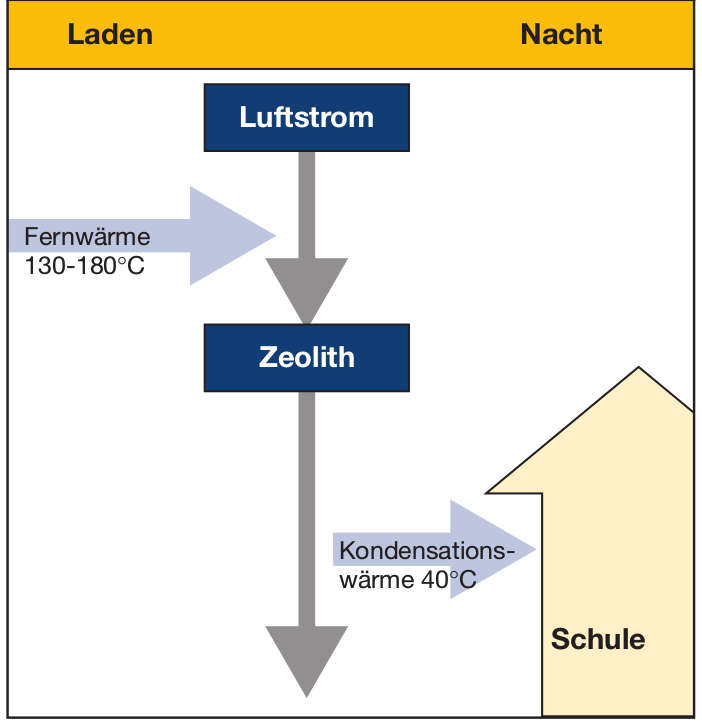
\includegraphics[scale=1]{images/Laden.jpg}
\caption{Laden des Zeolithspeichers \cite{BINE2}}
\label{fig:Laden}
\end{center}
\end{figure}

\begin{figure}[h!]
\begin{center}
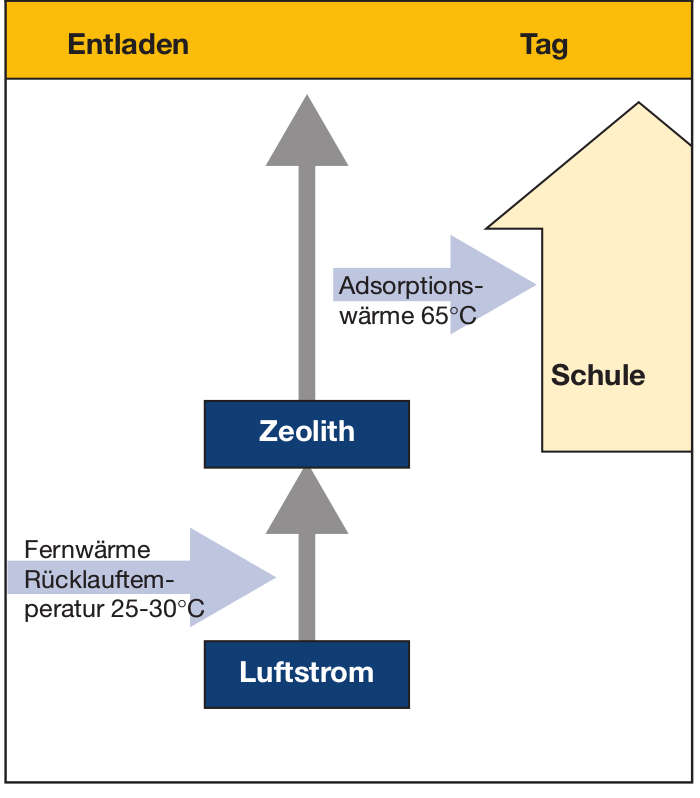
\includegraphics[scale=1]{images/Entladen.jpg}
\caption{Entladen des Zeolithspeichers \cite{BINE2}}
\label{fig:Entladen}
\end{center}
\end{figure}
Experimentell konnte ein Speicherwirkungsgrad von 86\% nachgewiesen werden.
Nachteilig erwiesen sich der hohe Preis von Zeolith der verhältnismässig hohe
Inverstitionskosten verursachte. Eine Ammortisation bei einem Betrieb mit 100
Zyklen pro Jahr scheint innert 10-15 Jahren möglich. Unter Laborbedingungen
verliert das Zeolith nach 100 Ladezyklen 15\% der Adsoprtionsenthalpie.
Anschliessend scheint die Adsorptionsfähigkeit des Stoffs stabil zu bleiben.
Dies ist ebenfalls in der Wirtschaftlichkeitsberechnung zu berücksichtigen.
\cite{BINE2}

\subsubsection{Saisonaler Speicher}
Saisonale thermochemische Speicher sind ebenfalls möglich. Das Fraunhofer-
Institut für solare Energiesysteme zusammen mit UFE Solar GmbH eine
Sorptionsspeicher für Niedrigenergiehäuser. Im Sommer word der Sorptionsspeicher
mittels thermischer Solarkollektoren aufgeladen und im Winter das Haus über den
Sorptionsspeicher mit thermischer Energie versorgt. Für Spitzenlastzeiten wurde
eine Zusatzheizung eingebaut. Als Speichermaterial wird handelsübliches
Silicagel verwendet. Technisch gesehen kommt auch hier ein Adsorptionsspeicher
mit kombinierter Wärmepumpe zum Einsatz. Das Prinzipschema ist in Abbildung \ref{fig:Saisonaler Speicher}
abgebildet.

\begin{figure}[h!]
\begin{center}
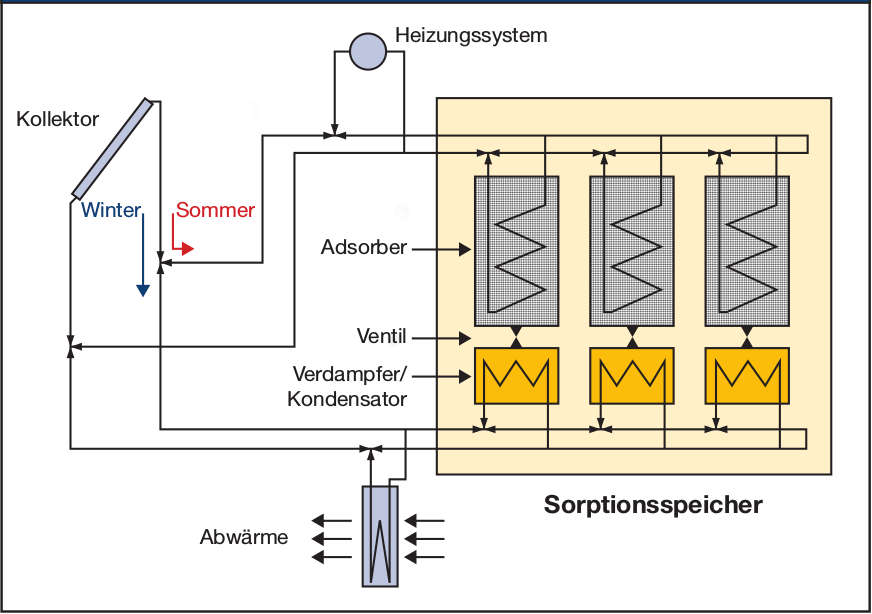
\includegraphics[scale=1]{images/energiehaus.jpg}
\caption{Schema des saisonalen chemischen Speichers \cite{BINE2}}
\label{fig:Saisonaler Speicher}
\end{center}
\end{figure}

Um einen möglichst flexiblen Einsatz mit gleichzeitiger Be- und Entladung zu
ermöglichen ist die geschlossen funktionierende Anlage drei Mal mit allen
Komponenten ausgestattet. Das Kondensat wird in dafür geeigneten Behältern
aufbewahrt. 

Anhand einer Simulation wurde die geschätzte Heizleistung von 4000kWh\/a mit
32m$^2$ thermischen Solarkollektoren und einem Sorptionsspeicher von 11m$^3$
Volumen veranschlagt bei 100\% Deckungsgrad. Ein Kostenoptimum für den solaren
Deckungsgrad mit Zusatzheizung wurde für eine Auslegung 80-90\% prognostiziert.

Zum Zeitpunkt der Publikation von \cite{BINE2} befindet sich der Speicher noch
in Evaluation. Insbesondere der tatsächlich erreichbare solare Deckungsgrad wäre
dabei von Interesse. Leider liessen sich im Internet keine aktualiserten
Resultate zu diesem Projekt finden.
\subsection{Latentspeicher}
Die Zürcher Firma GLASSX stellt PCM Fassadenelemente her. 

Kernprodukte sind
GLASSX\circledR store, ein kombinierbares Innenelement für Gebäude mit
Glassfassade und GLASSX\circledR crystal, ein Komplettfasadenelement mit
Verschattung und Dämmung für Leichtbaugebäude. Die beiden Produkte besitzen eine
ähnlichen Aufbau. Das PCM, Kalziumchloridhexahydrat (\ce{CaCl_2\cdot 6H_2O}),
liegt zwischen zwei Gläsern in der Mitte des Elements. Der Schmelzpunkt von
\ce{CaCl_2\cdot 6H_2O} liegt genau bei Raumtemperatur (Salzhydrat). Bei
Erwärmung durch Sonneneinstrahlung schmilzt das \ce{CaCl_2\cdot 6H_2O} und
entzieht so der Umgebung Wärme. Bei Abkühlung in der Nacht gestaltet sich der
Prozess genau umgekehrt. \ce{CaCl_2\cdot 6H_2O} erstarrt und gibt Wärme an die
Umgebung ab. Da diese Elemente als Fassade bzw. direkt hinter der GLasfassade
eingesetzt werden, wird bicht nur Raumwärme sondern auch die Einstrahlungswärme
der Sonne genutzt. Infrarotstrahlung wird durch das PCM fast komplett
absorbiert, für sichtbares Licht ist das Material zum grössten Teil durchlässig.
Als weitere Innovation hat das Unternehmen ein Prismenglas entwickelt, dass die
unterschiedlichen Einstrahlungswinkel während der Jahreszeiten als Selektion
nutzt. Bei hohen Einstrahlungswinkeln wie sie im Sommer vorkommen wird über
Totalreflexion der grösste Teil der Strahlung bereits im Prismenglas absorbiert.
Im Winter bei niedrigeren Einstrahlungswinkeln lässt das Glas die Strahlung
annähernd verlustfrei durch. Somit sind im Winter solare Gewinne möglich. In
Abbildung \ref{fig:glassx schema} ist das Schema einer GLASSX\circledR crystal
Fassade mit Prismenglas abgebildet. 

\begin{figure}[h!]
\begin{center}
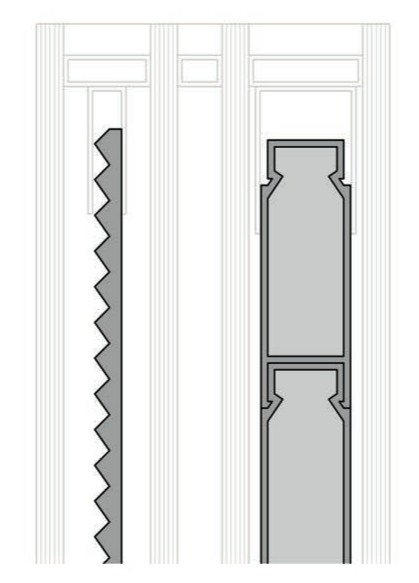
\includegraphics[scale=0.7]{images/glassxcrystal.jpg}
\caption{Schema einer GLASSX\circledR crystal Fassade \cite{glassxbr}}
\label{fig:glassx schema}
\end{center}
\end{figure}

Der Autor konnte sich im Referenzgebäude von Marché Schweiz selber auf einer
Exkursion von der Funktionalität der Elemente überzeugen. Die Wirkung dieser
Bauteile ist bestechend. Das Raumklima blieb ohne zusätzliche Verschattung
selbst im Hochsommer angenehm. Als Ergänzung zu den baulichen Massnahmen wurde
die Luftbefeuchtung mit speziellen Wasserpflanzen gewährleistet. 
\newpage
\section{Ausblick}

\listoftables
\newpage
\listoffigures
\newpage
\begin{thebibliography}{99}
	\bibitem{BINE1}BINE Energieforschung für die Praxis. Abgerufen am 11.04.2014
	von http://www.bine.info/typo3temp/pics/b193b0972c.gif verändert durch D. Strebel
	\bibitem{Wesselak}Wesselak et. al. Regenerative Energiesysteme. 2. Auflage.
	Springer Vieweg Verlag Berlin. 2013
	\bibitem{Hiebler} Hiebler S. Kalorimetrische Methoden zur Bestimmung der
	Enthalpie von Latentwärmespeichermaterialien während des Phasenübergangs. Dissertation.
	München. 2007
	\bibitem{BINE2} BINE Energieforschung für die Praxis. projektinfo 2\/01
	Thermochemische Speicher. 2001
	\bibitem{glassxbr} GLASSX\circledR crystal. Das Glas, das speichert, wärmt und
	kühlt. Produktbroschüre. Zürich. 2005. 
	\bibitem{Phasendiagramm} Wikipedia Phasendiagramm. 
	
	Abgerufen von
	http//commons.wikimedia.org/wiki/File:Phasendiagramme.svg am 28.04.2014.
	Verändert von D.Strebel
\end{thebibliography}
\end{document}
